\documentclass[aspectratio=169]{beamer}
\usepackage{animate}
\usepackage{tikz}
\usetheme{metropolis}

% Bibliography setup
\usepackage{natbib}
\bibliographystyle{apalike}

\title{Bayesian anomaly detection}
\date{January 21, 2025}
\author{Samuel Alan Kossoff Leeney, Will Handley, Dominic Anstey, Eloy de Lera Acedo}
\institute{Will Handley's group meeting}
\begin{document}
\begin{frame}
  \titlepage
\end{frame}

\begin{frame}{What is anomaly detection useful for?}
  \begin{columns}
    \begin{column}{0.5\textwidth}
        \textbf{1. Contamination}
        \begin{itemize}
          \item Simultaneously detecting and mitigating contaminated data.
        \end{itemize}
    \end{column}
    \begin{column}{0.5\textwidth}
        \textbf{2. Anomalies}
        \begin{itemize}
          \item Radio transients, cosmic ray flares, GW signals etc.)
        \end{itemize}
    \end{column}
  \end{columns}
\end{frame}

\begin{frame}{Contaminated data}
  \begin{figure}
    \centering
    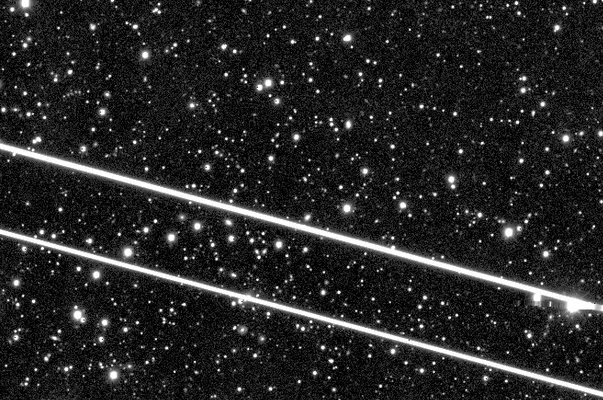
\includegraphics[width=\textwidth]{images/starlink2.png}
  \end{figure}
\end{frame}

\begin{frame}{Contaminated data on the REACH site}
  \begin{figure}
    \centering
    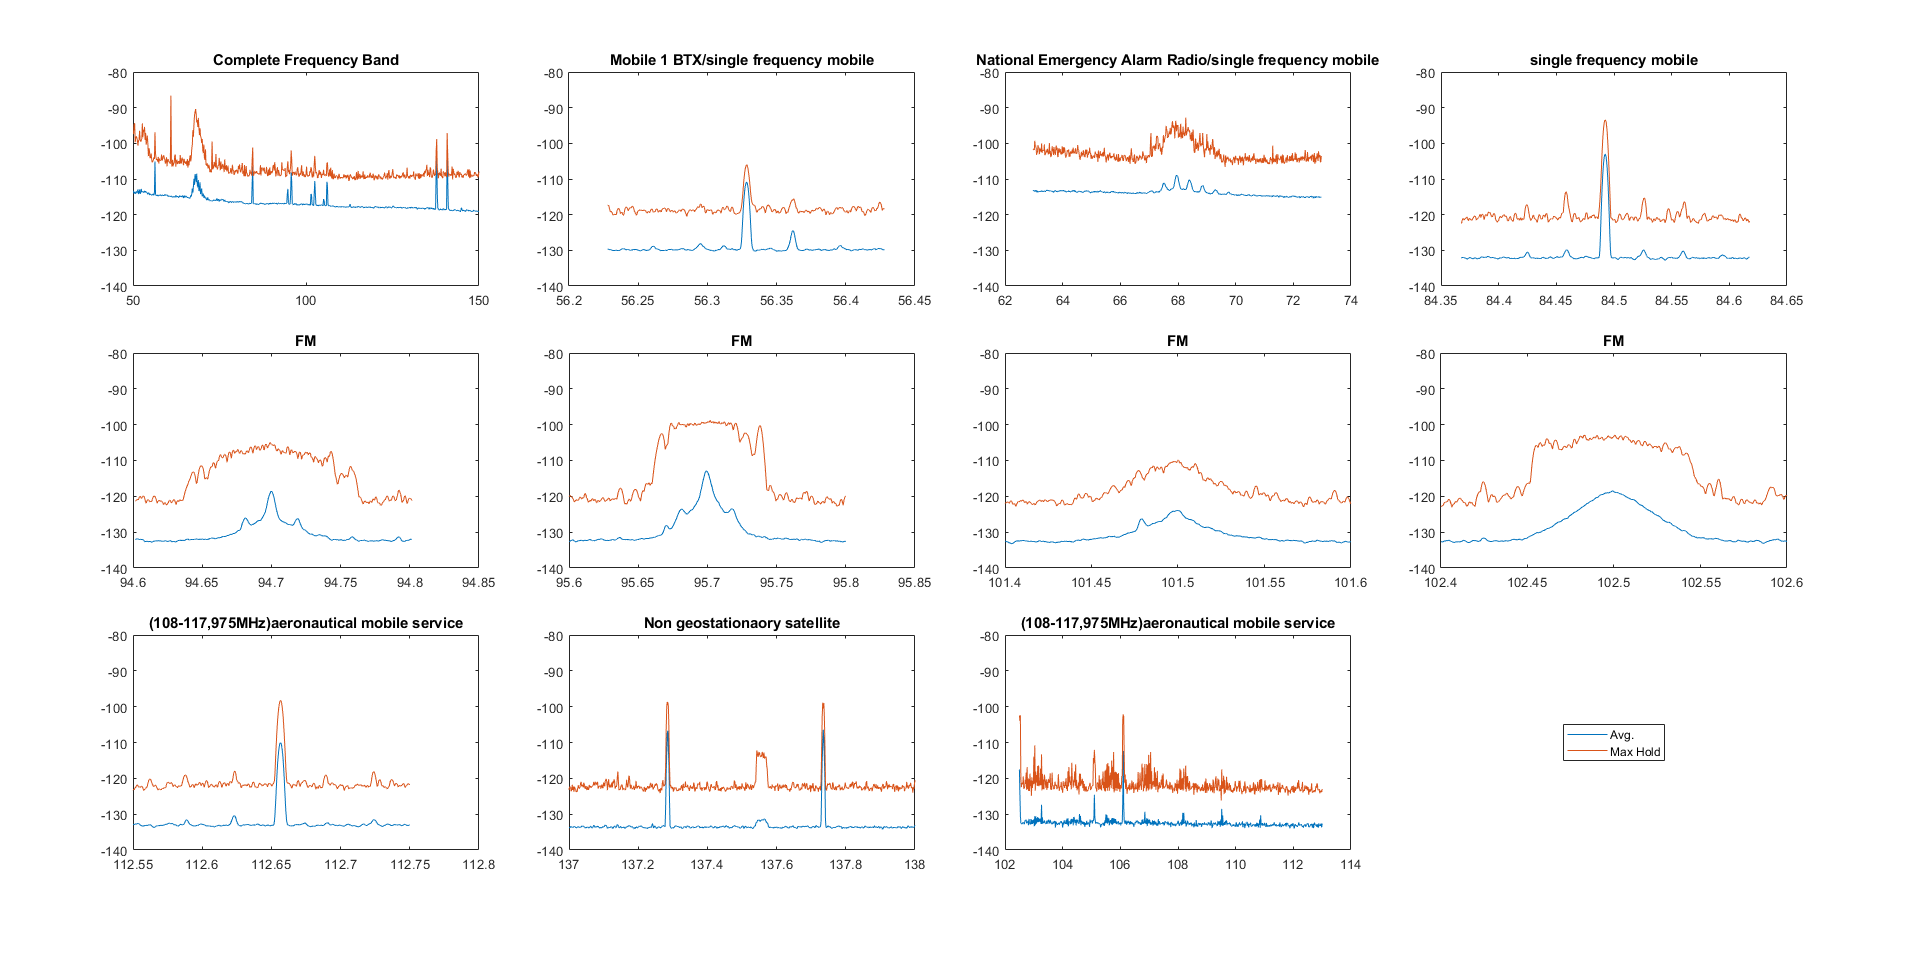
\includegraphics[width=\textwidth]{images/rfi_site.png}
  \end{figure}
\end{frame}

\begin{frame}{Anomalies - FRB 1}
  \centering
  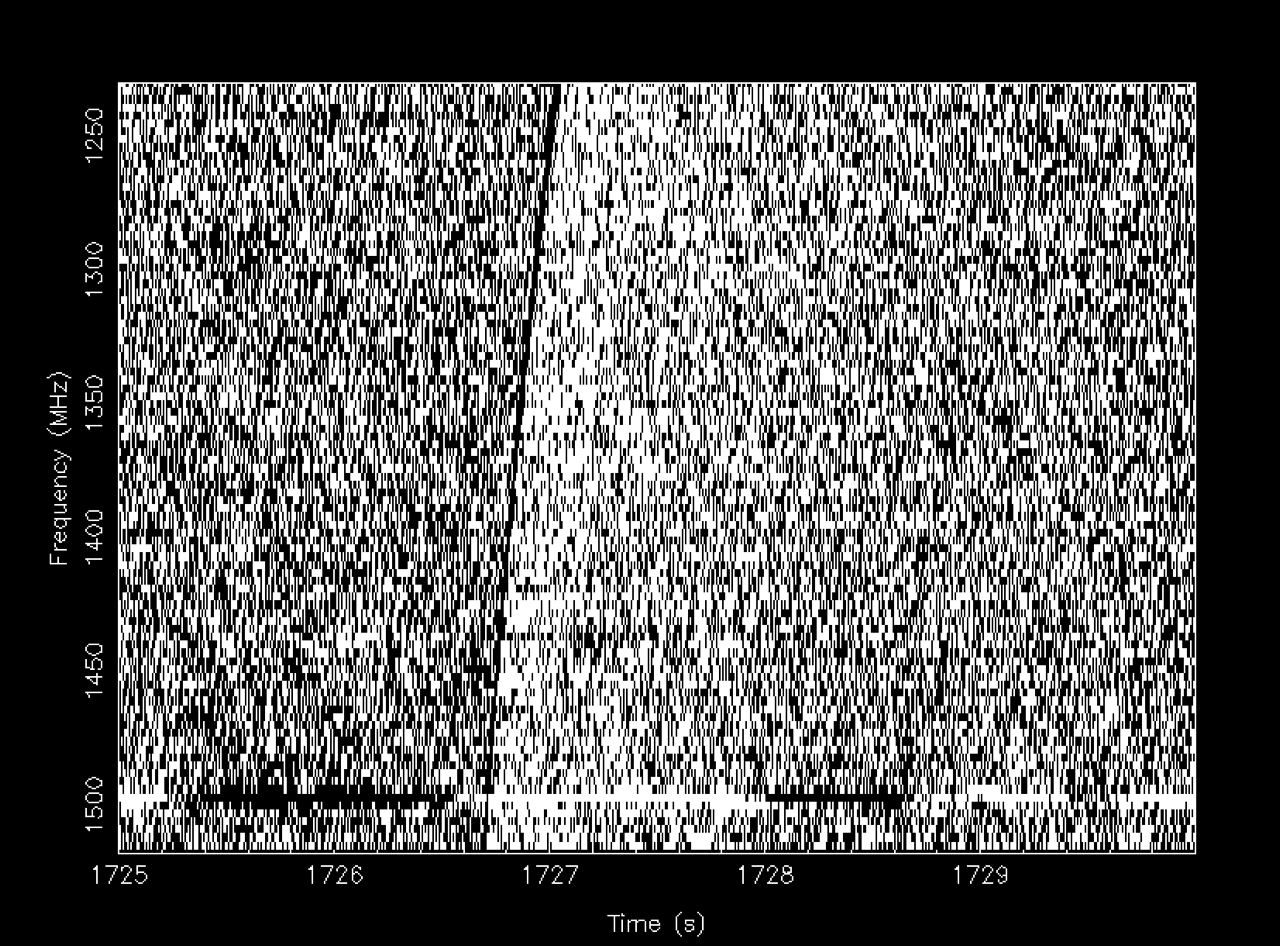
\includegraphics[width=0.8\textwidth]{images/Frb_1.png}
\end{frame}

\begin{frame}{Anomalies (GW150914)}
  \centering
  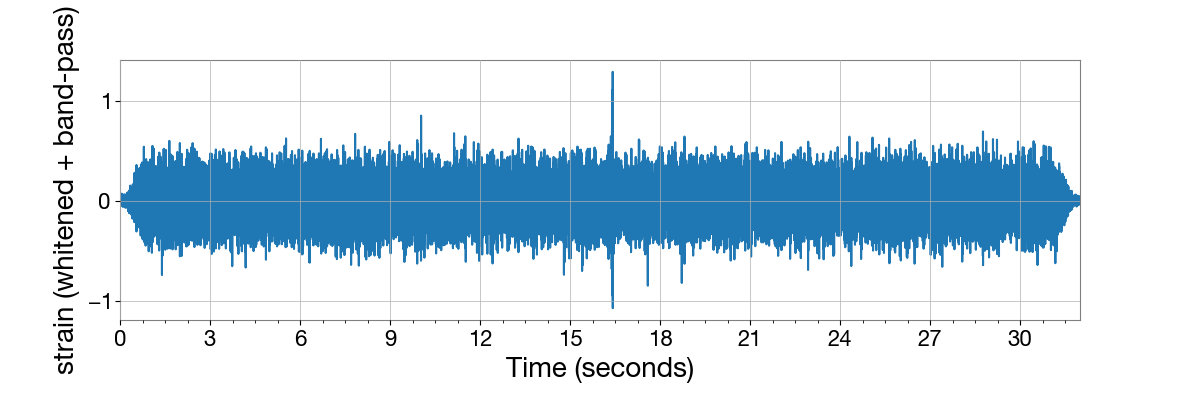
\includegraphics[width=\textwidth]{images/gwanomaly.png}
\end{frame}

\begin{frame}{What do(nt) we look for?}
  \centering
  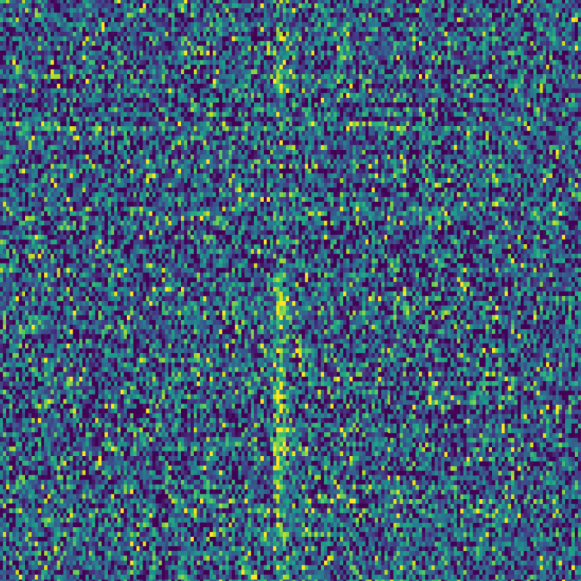
\includegraphics[width=0.8\textwidth]{images/frb.png}
\end{frame}

\begin{frame}{Over simplified example of anomaly detection method (thresholding)}
  \footnotesize
  \textbf{Simple statistical approach:}
  \begin{itemize}
    \item Calculate mean ($\mu$) and standard deviation ($\sigma$) of the data
    \item Define threshold $T = \mu + k\sigma$ where $k$ is a sensitivity parameter
    \item Flag data point $x_i$ as anomalous if:
  \end{itemize}
  \begin{equation}
    \text{anomaly}_i = \begin{cases}
      1 & \text{if } x_i > T \\
      0 & \text{otherwise}
    \end{cases}
  \end{equation}
  \textbf{Limitations:}
  \begin{itemize}
    \item Choice of $k$ is arbitrary
    \item Assumes Gaussian statistics
    \item No consideration of temporal correlations
    \item Cannot distinguish between RFI and real signals
  \end{itemize}
\end{frame}

\begin{frame}{Thresholding results}
  \begin{columns}
    \column{0.5\textwidth}
    \textbf{Constant signal with RFI:}
    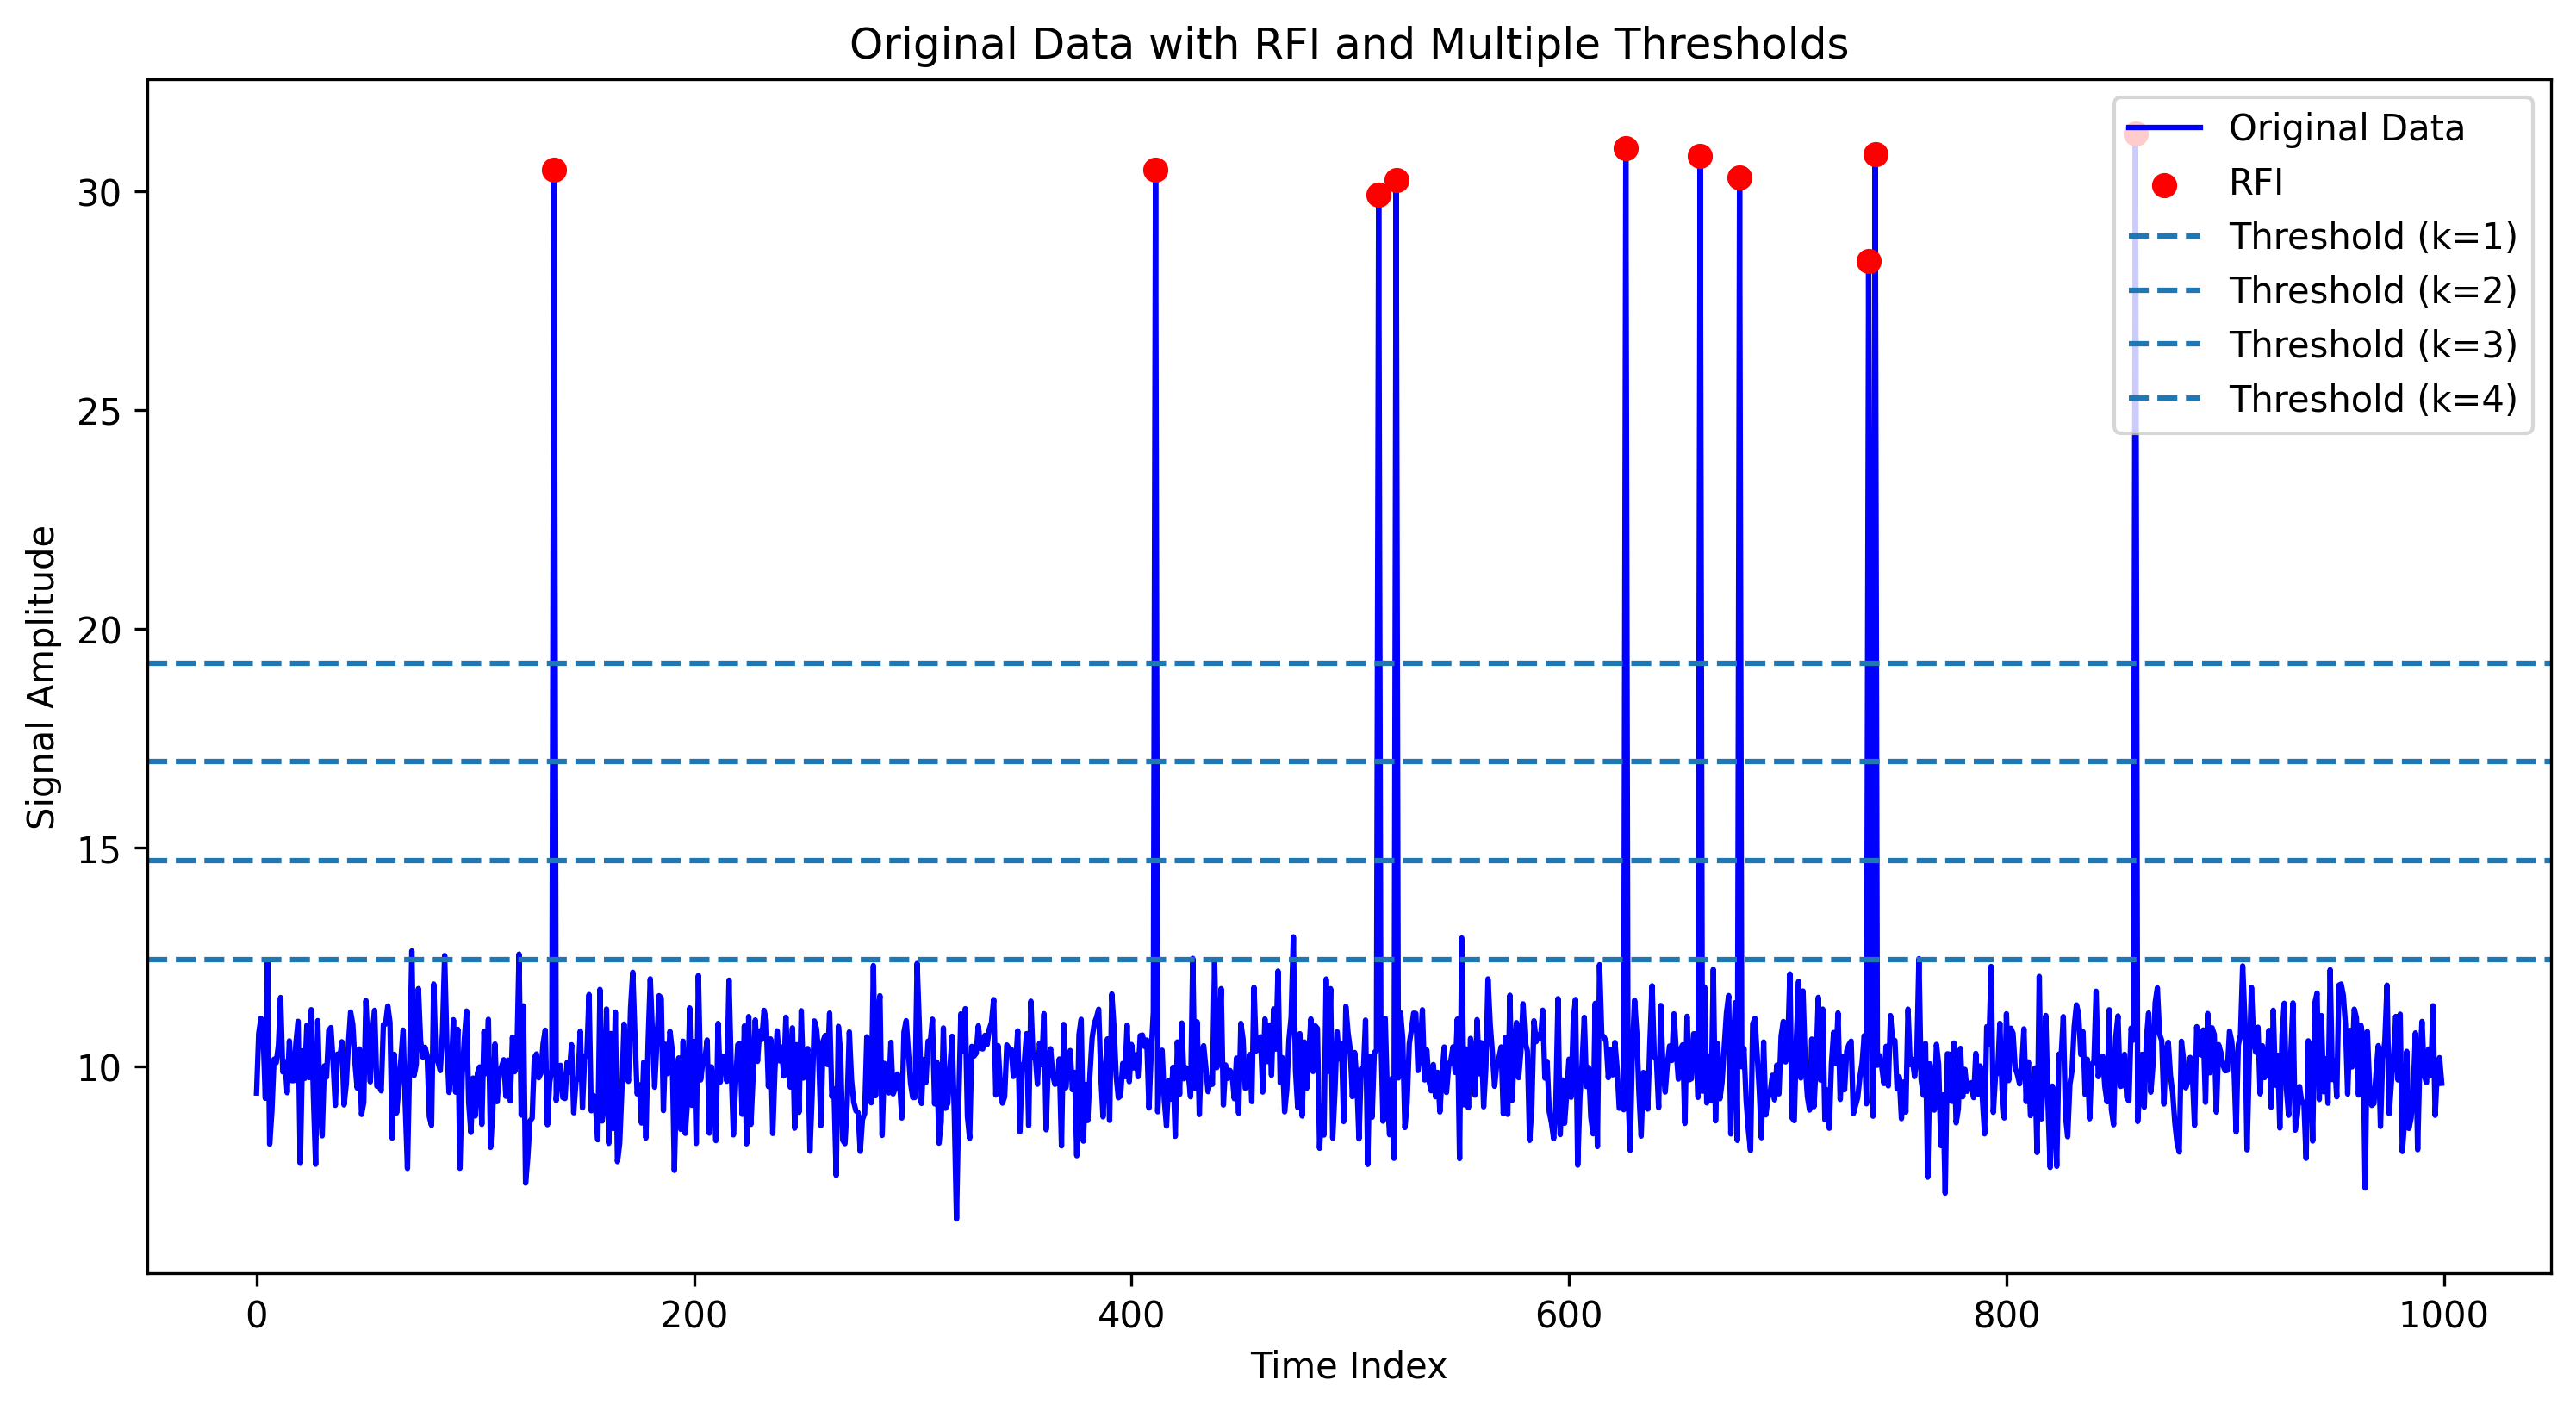
\includegraphics[width=\textwidth]{images/threshold_multiple.png}
    \column{0.5\textwidth}
    \textbf{Sine wave with RFI:}
    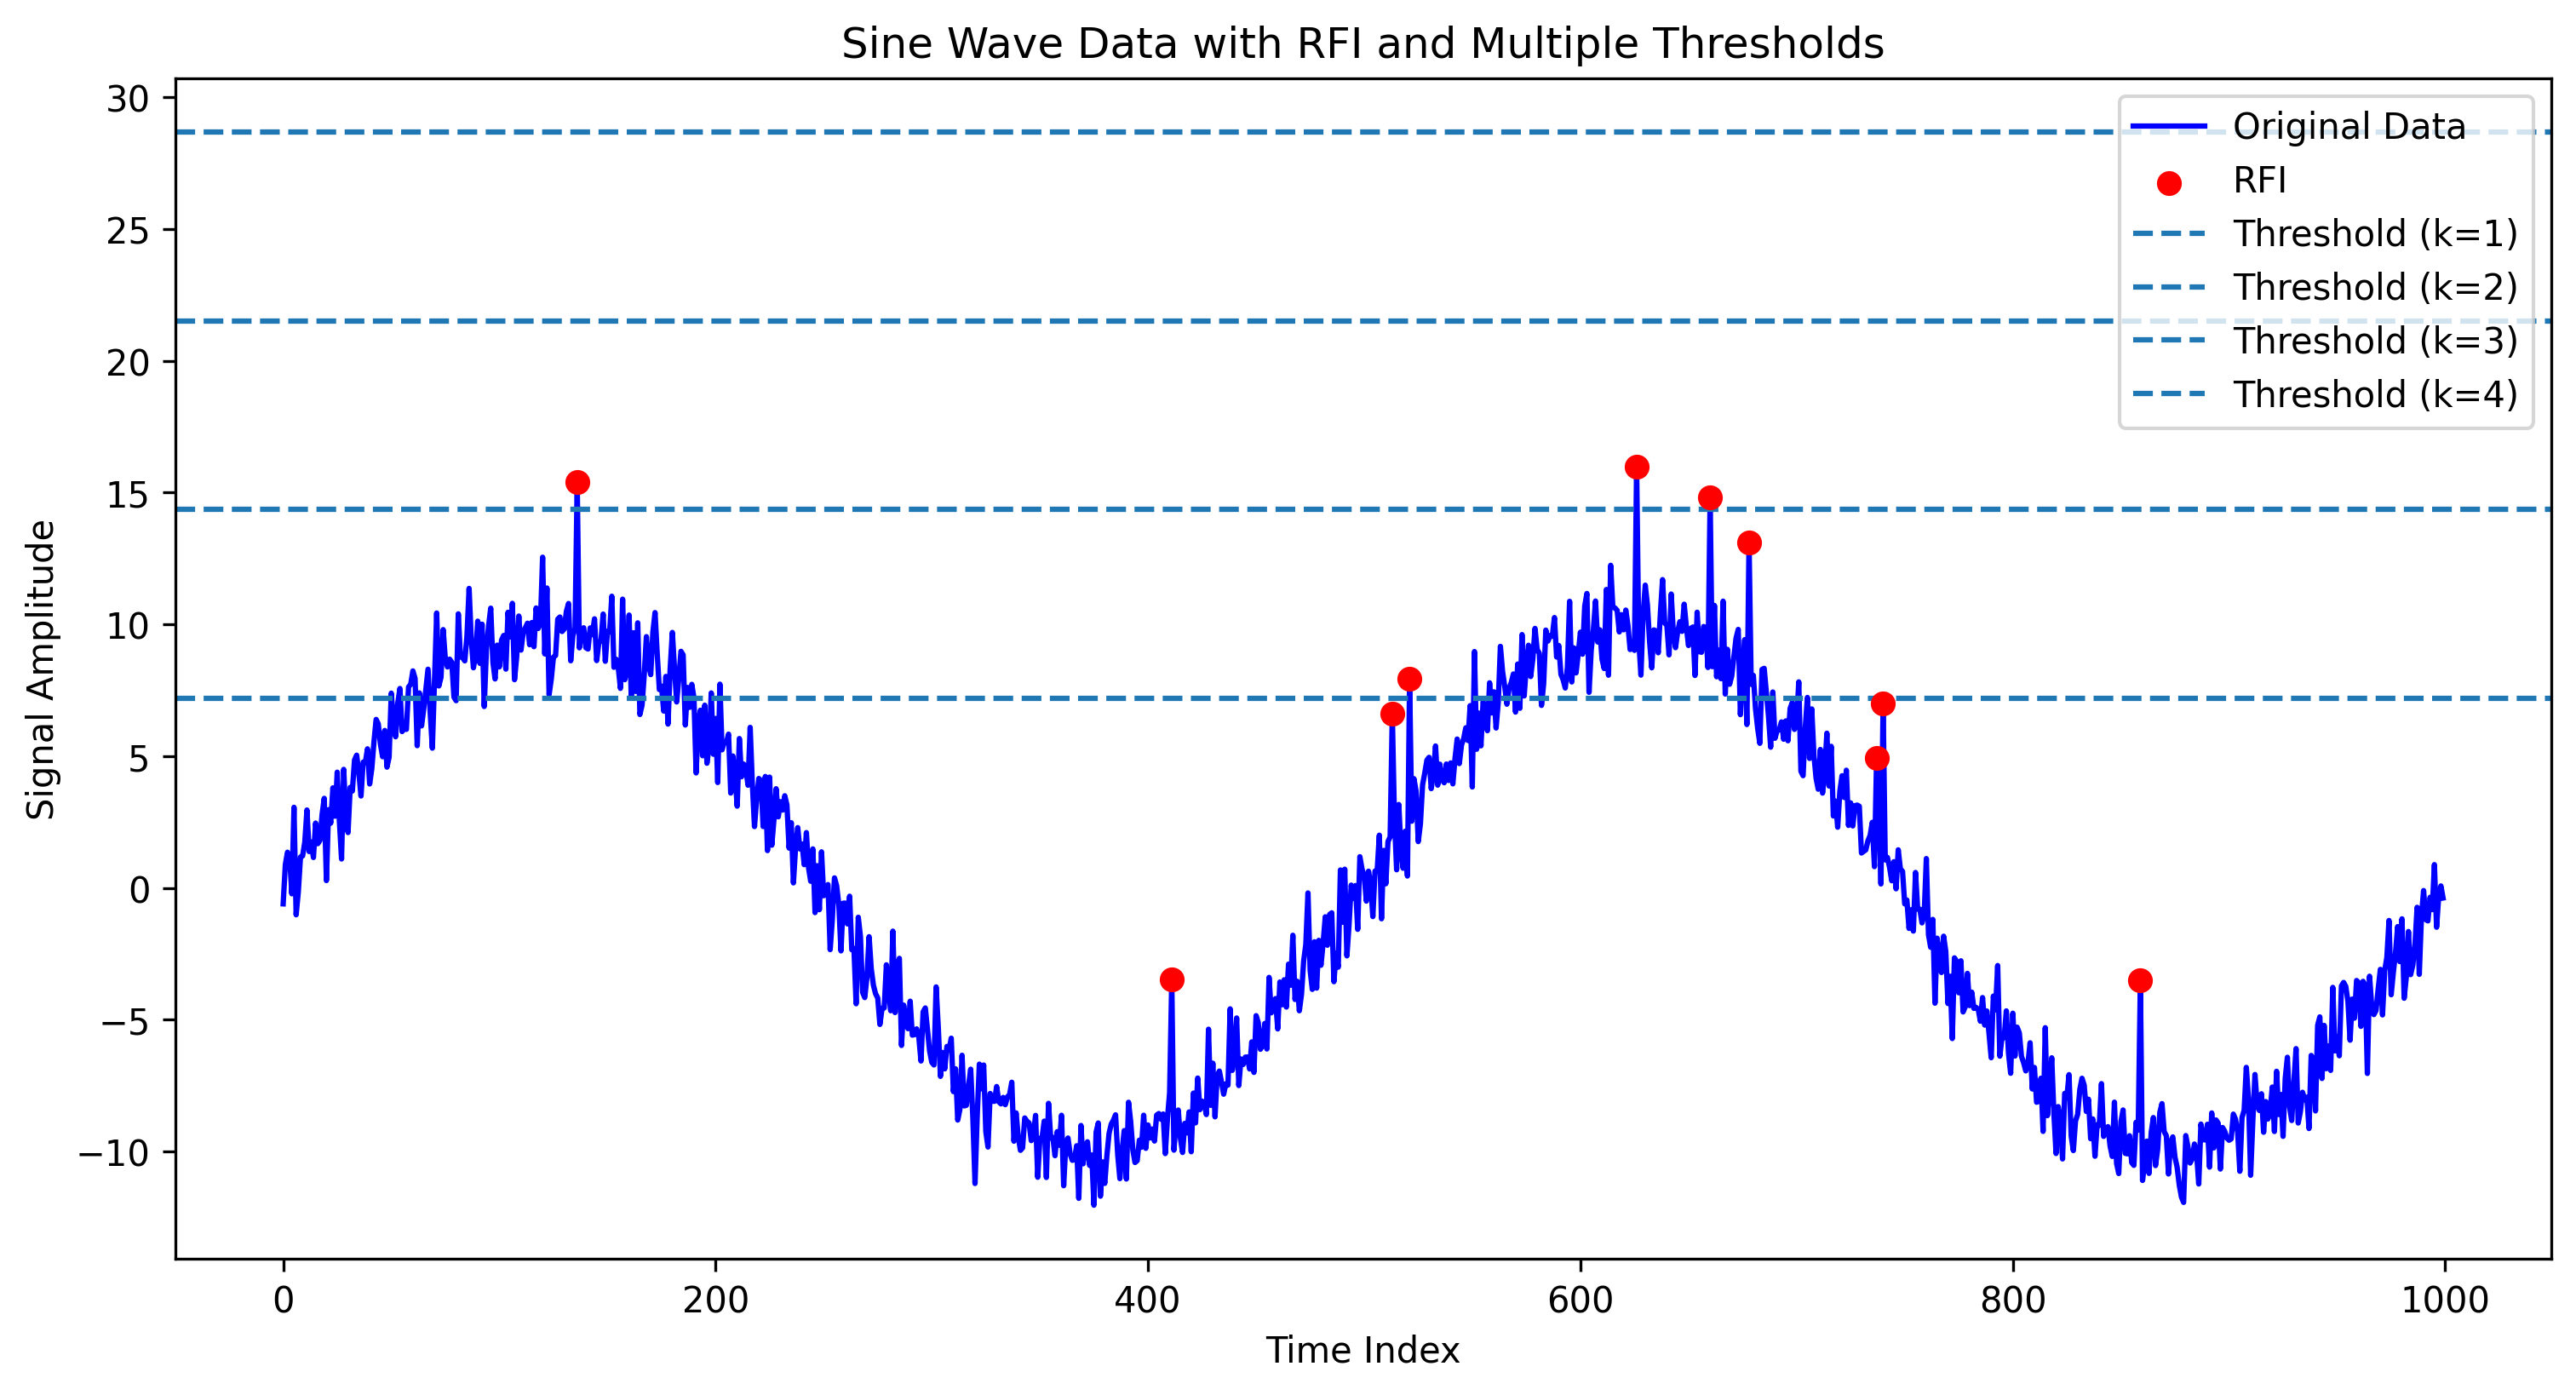
\includegraphics[width=\textwidth]{images/threshold_sin_multiple.png}
  \end{columns}
\end{frame}

\begin{frame}{Defining an anomaly sensitive likelihood}
  \footnotesize
  \textbf{a) Generate peicewise likelihood:}
  \begin{equation}
      P(\mathcal{D}_i|\theta) = \begin{cases}
          \mathcal{L}_i(\theta) &: \text{expected}\\
          \Delta^{-1}[ 0<\mathcal{D}_i<\Delta] &: \text{anomalous},
      \end{cases}
  \end{equation}

  \textbf{b) Ascribe Bernoulli prior:}
  \begin{equation}
      P(\varepsilon_i) = p_i^{(1-\varepsilon_i)}(1-p_i)^{\varepsilon_i}.
  \end{equation}

  \textbf{c) Marginalise over epsilon:}
  \begin{equation}
      P(\mathcal{D} | \theta) =\sum_{\varepsilon \in \{ 0, 1 \} ^N}P(\mathcal{D},\varepsilon|\theta)
    \end{equation}


    \textbf{d) Approximate correct mask is most likely}
     \begin{equation}
 P(\mathcal{D}|\theta, \varepsilon_{\mathrm{max}}) \gg \mathrm{max}_j P(\mathcal{D}|\theta,\varepsilon^{(j)})\label{eq:nlo},
\end{equation}

  \textbf{e) Loglikelihood:}
  \begin{equation}
      \log{P(\mathcal{D}|\theta)} = \sum_{i}[{\log{\mathcal{L}_i}+\log({1-p_i})]\varepsilon^{\mathrm{max}}_i + [\log{p}_i - \log{\Delta}](1 - \varepsilon^\mathrm{max}_i})
  \end{equation}
\end{frame}

\begin{frame}{Computing the Posterior}
    \footnotesize
    \textbf{e) Loglikelihood:}
  \begin{equation}\tag{6}
      \log{P(\mathcal{D}|\theta)} = \sum_{i}[{\log{\mathcal{L}_i}+\log({1-p_i})]\varepsilon^{\mathrm{max}}_i + [\log{p}_i - \log{\Delta}](1 - \varepsilon^\mathrm{max}_i})
  \end{equation}

    \footnotesize
    \textbf{f) Maximise $\varepsilon^{max}$ by comparing the terms:}
    \begin{equation}\tag{7}
    \log P(\mathcal{D}|\theta) =
    \begin{cases} 
    \log \mathcal{L}_i + \log(1 - p_i), & \text{if } [\log \mathcal{L}_i + \log(1 - p_i) > \log p_i - \log \Delta] \\
    \log p_i - \log \Delta, & \text{otherwise}
    \end{cases}
    \end{equation}
\end{frame}

\begin{frame}{Fit on a simple toy model}
    \centering
    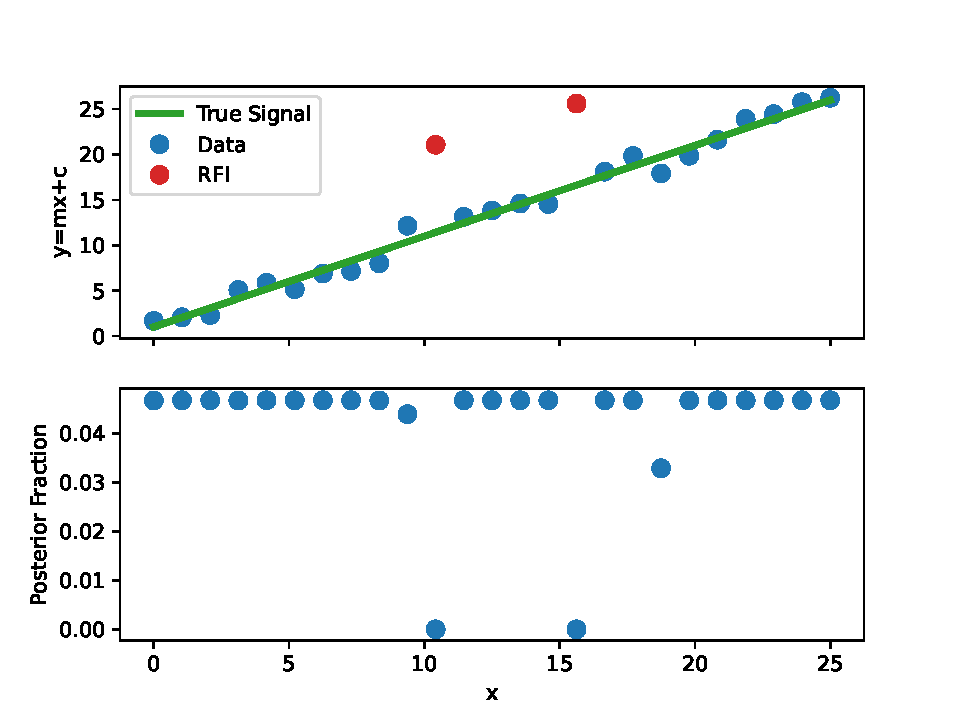
\includegraphics[width=0.7\textwidth]{images/test.pdf}
  \end{frame}

\begin{frame}{Likelihood thresholding condition $p$}
    \begin{equation}
    \begin{aligned}
    \log{P(\mathcal{D}|\theta)} &= \sum_{i}[{\log{\mathcal{L}_i}+\log({1-p_i})]\varepsilon^{\mathrm{max}} + [\log{p}_i - \log{\Delta}](1 - \varepsilon^\mathrm{max}_i})\label{eq:loglikelihood}
    \end{aligned}
    \end{equation}
    \centering
    \animategraphics[autoplay,loop,width=11cm]{2}{images/gif_anest/comb_}{1}{9}
\end{frame}

\begin{frame}{Varying $p$}
    \centering
    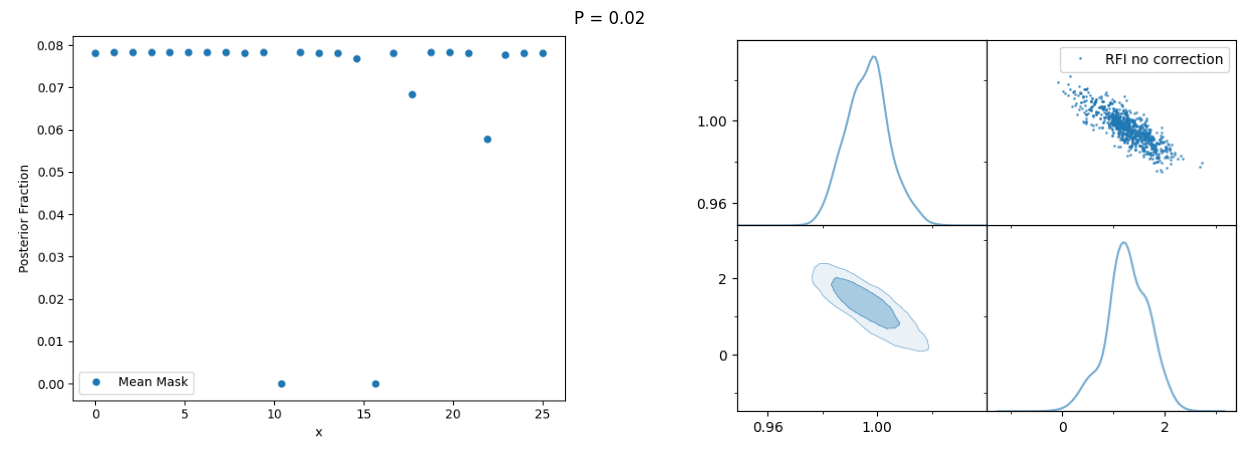
\includegraphics[width=\textwidth]{images/gif_anest/comb_2.png}
\end{frame}

\begin{frame}{Varying $p$}
    \centering
    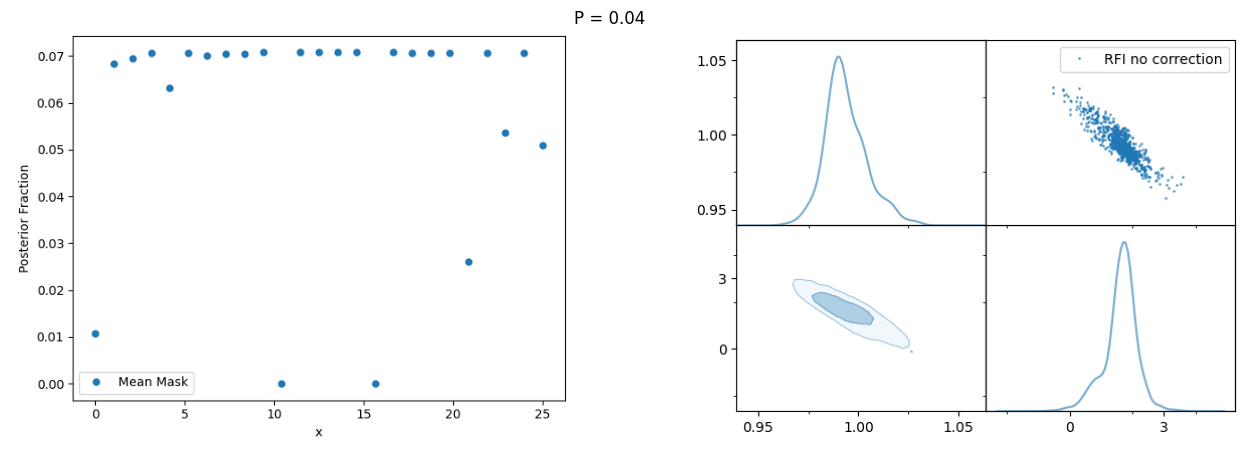
\includegraphics[width=\textwidth]{images/gif_anest/comb_3.png}
\end{frame}

\begin{frame}{Varying $p$}
    \centering
    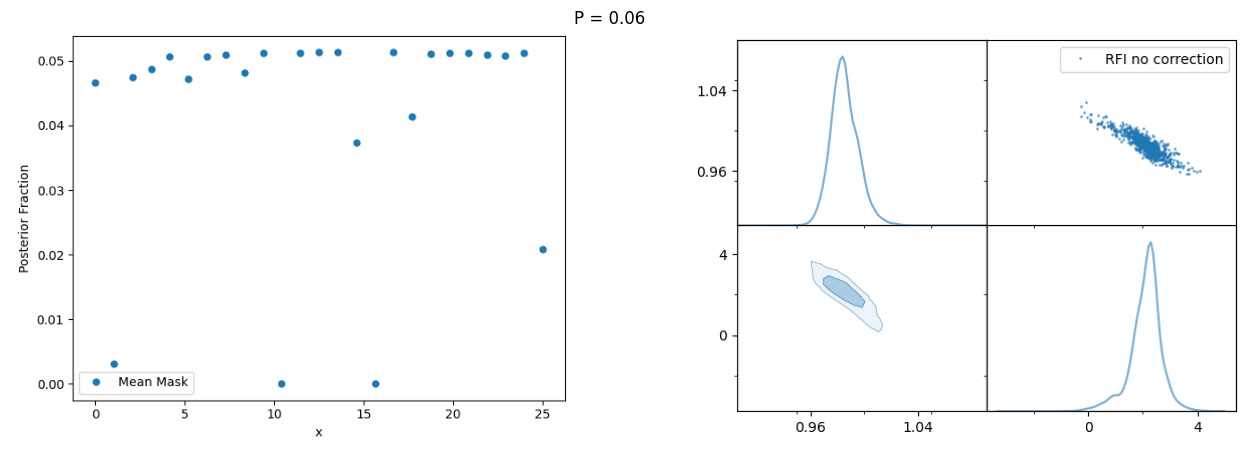
\includegraphics[width=\textwidth]{images/gif_anest/comb_4.png}
\end{frame}

\begin{frame}{Varying $p$}
    \centering
    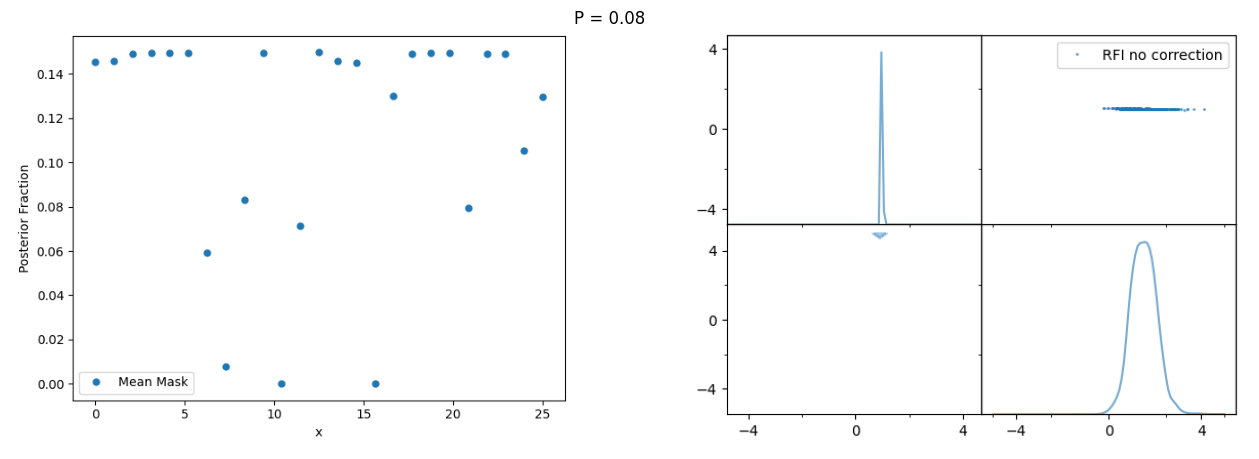
\includegraphics[width=\textwidth]{images/gif_anest/comb_5.png}
\end{frame}

\begin{frame}{Varying $p$}
    \centering
    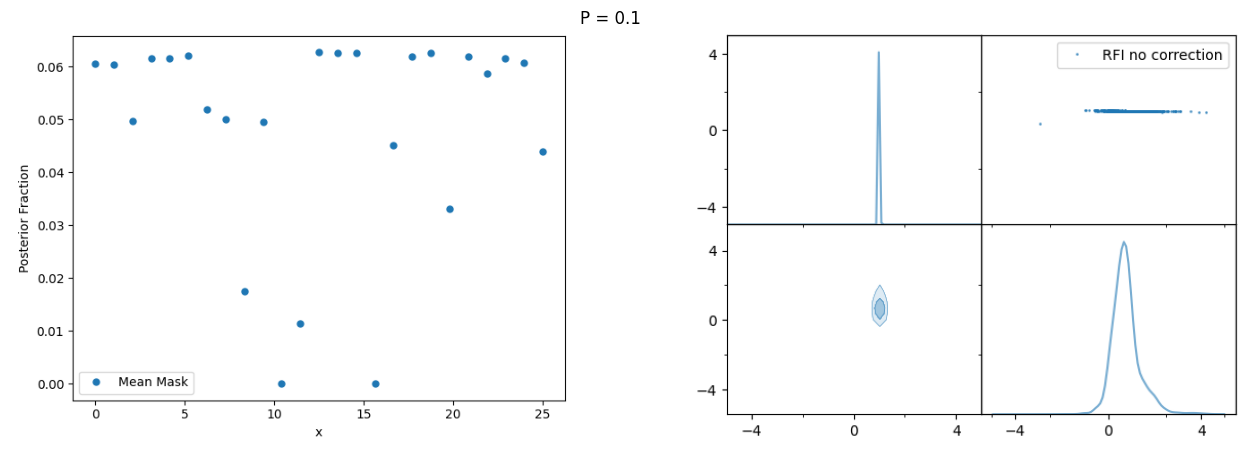
\includegraphics[width=\textwidth]{images/gif_anest/comb_6.png}
\end{frame}

\begin{frame}{Varying $p$}
    \centering
    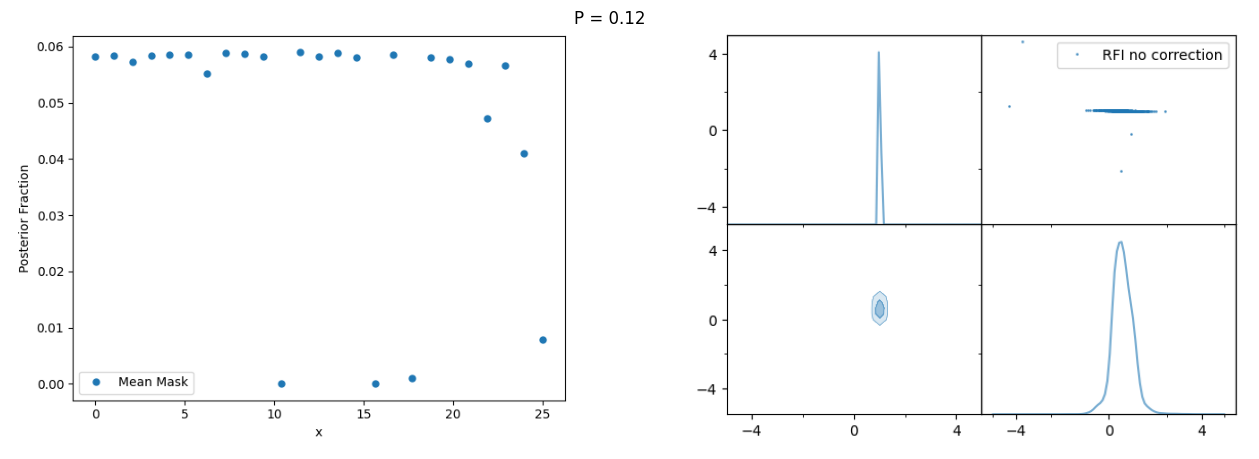
\includegraphics[width=\textwidth]{images/gif_anest/comb_7.png}
\end{frame}

\begin{frame}{Varying $p$}
    \centering
    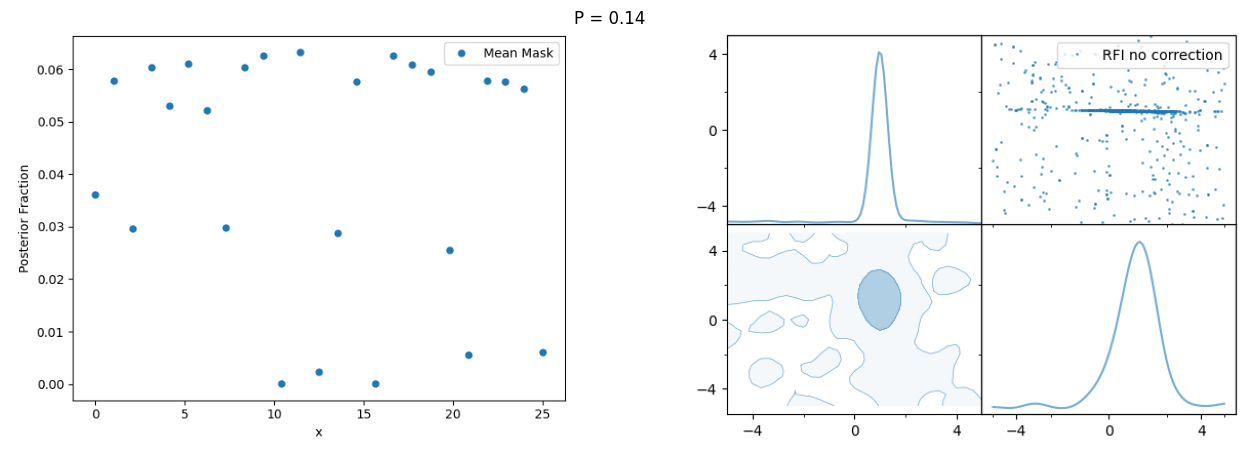
\includegraphics[width=\textwidth]{images/gif_anest/comb_8.png}
\end{frame}

\begin{frame}{Varying $p$}
    \centering
    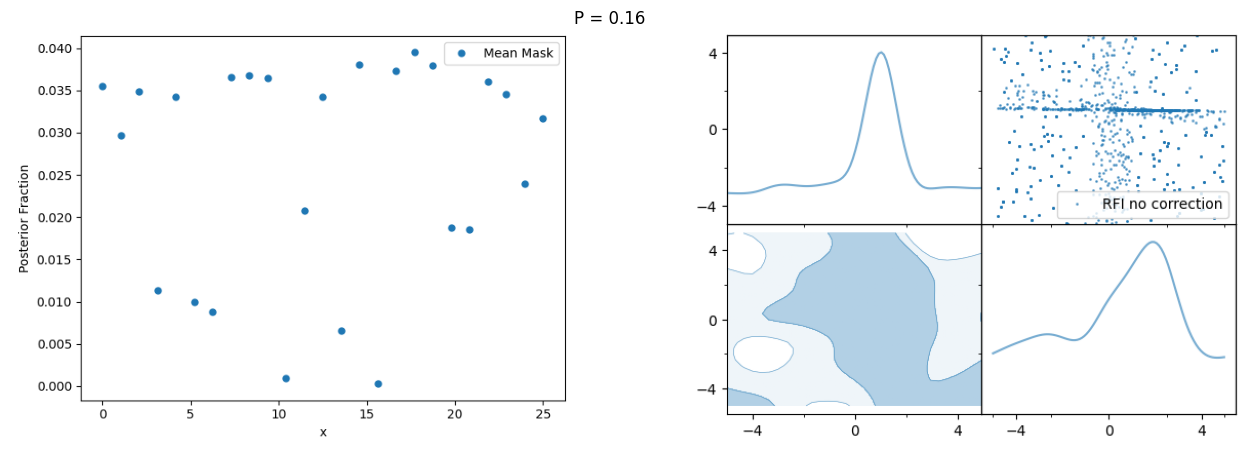
\includegraphics[width=\textwidth]{images/gif_anest/comb_9.png}
\end{frame}

  \begin{frame}{Selection strategy for $p$.}
    \begin{columns}
      \column{0.5\textwidth}
      \begin{itemize}
        \item `Select $p$ such that the Bayesian evidence is maximised'
      \end{itemize}
      \column{0.5\textwidth}
      \begin{figure}
        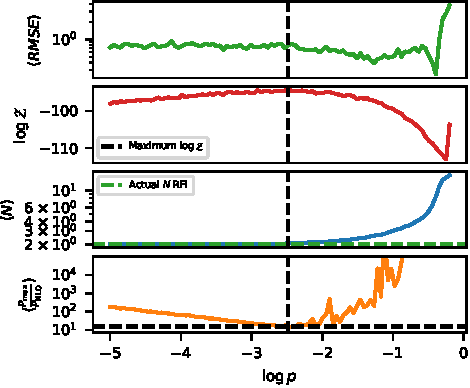
\includegraphics[width=1.1\textwidth]{images/f_approx_current_sig5_2.pdf}
      \end{figure}
    \end{columns}
  \end{frame}


  \begin{frame}{Fully automated anomaly detection}
    \begin{itemize}
    \item Putting a prior on $p$, we can fit it dynamically as a free parameter.
    \item This fully automates the anomaly detection process.
    \item Must exclude $p=0$.
    \end{itemize}
\end{frame}

\begin{frame}{Application to toy model}
    \centering
    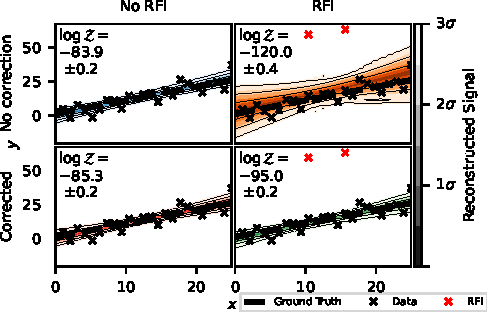
\includegraphics[width=0.9\textwidth]{images/4pane_toy_sidebar.pdf}
\end{frame}

\begin{frame}{Application to REACH data}
    \centering
    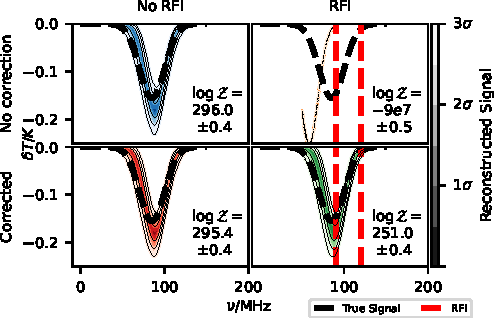
\includegraphics[width=0.9\textwidth]{images/4pane_reach_sidebar.pdf}
\end{frame}

\begin{frame}{Implement with 2 lines of code}
    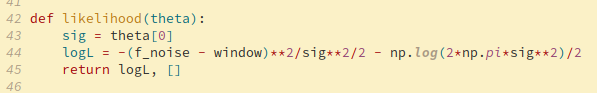
\includegraphics[width=1\textwidth]{images/logl1.png}
    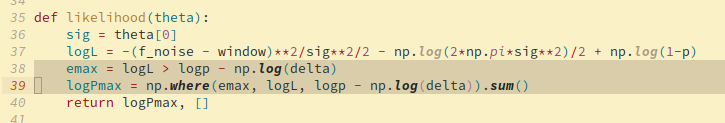
\includegraphics[width=1\textwidth]{images/logl2.png}
    \centering Tutorial @ github.com/samleeney
\end{frame}

\begin{frame}{Problems with this method}
    \begin{itemize}
        \item Requires some knowledge of a real model for the data
        \begin{itemize}
            \item Cannot be used as a blind search tool
            \item Model must be reasonably accurate
        \end{itemize}
        \item Currently struggling to detect RFI on REACH
        \begin{itemize}
            \item Not at noise level for 21cm signal
            \item Signal-to-noise ratio affects detection efficiency
        \end{itemize}
        \item Implementation challenges
        \begin{itemize}
            \item Requires existing Bayesian pipeline
            \item Can be difficult to integrate into established projects
            \item Computational overhead may be significant
        \end{itemize}
    \end{itemize}
\end{frame}

\begin{frame}{Read the paper!}
  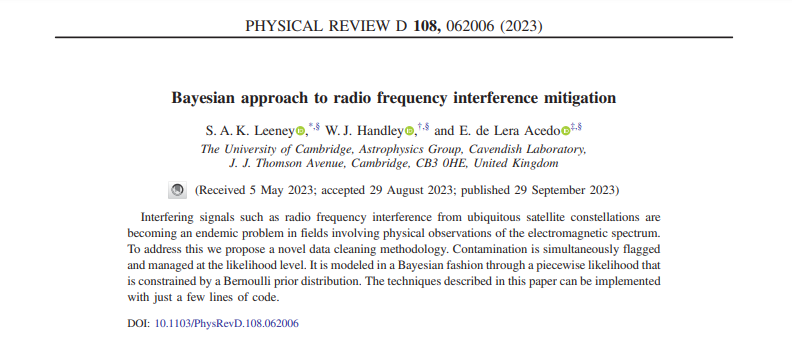
\includegraphics[width=1\textwidth]{images/paper1.png}
  \href{https://arxiv.org/abs/2211.15448}{arxiv: 2211.15448}
\end{frame}

\section{A new use case: supernovae anomaly detection}

\begin{frame}{SALT and SNooPy Models}
    \begin{columns}[t] % Align columns at the top
        \column{0.5\textwidth}
        \footnotesize
        \textbf{SALT Model:}
        \[
            F(p, \lambda) = x_0 \left[ M_0(p, \lambda) + x_1 M_1(p, \lambda) + \ldots \right] 
            \]
            \[
            \times \exp \left[ c \times CL(\lambda) \right]
        \]
        Where:
        \begin{itemize}
            \item Free parameters are: $x_0$, $x_1$, $t_0$, and $c$
            \item Model surface parameters are: $M_0(p, \lambda)$, $M_1(p, \lambda)$
            \item $p$ is a function of redshift and $t_0$
        \end{itemize}
        
        \column{0.5\textwidth}
        \footnotesize
        \textbf{SNooPy Model:}
        \begin{itemize}
            \item Uses empirical templates with shape parameters ($\Delta m_{15}$ or $s_{BV}$)
            \item Models host galaxy extinction using reddening laws
        \end{itemize}
    \end{columns}
\end{frame}

\begin{frame}{Light Curve Image}
    \centering
    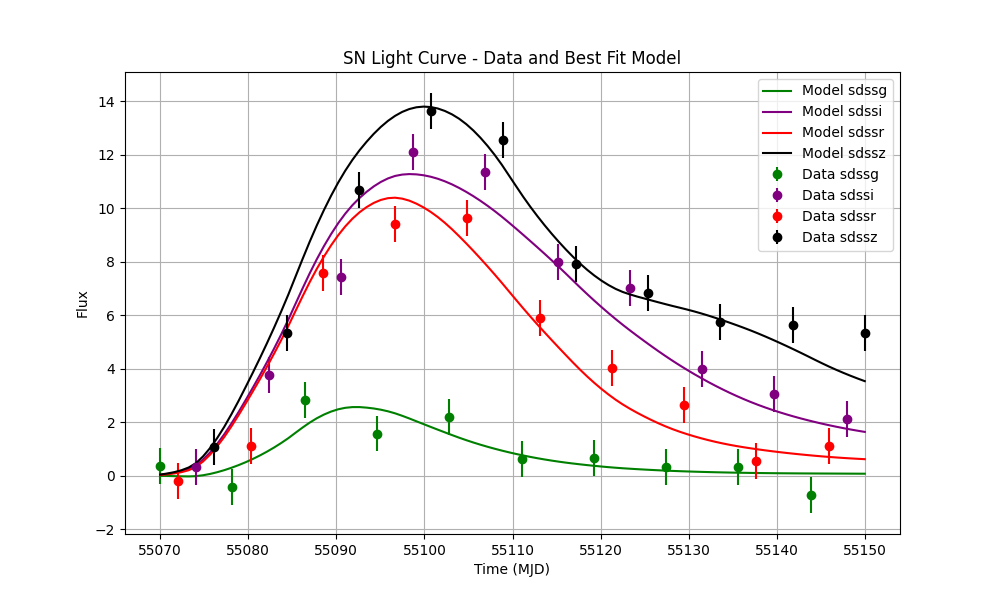
\includegraphics[width=\textwidth]{images/sncosmo-fitter.png}
\end{frame}

\begin{frame}{Anomaly detection by comparing SALT and SNooPy}
    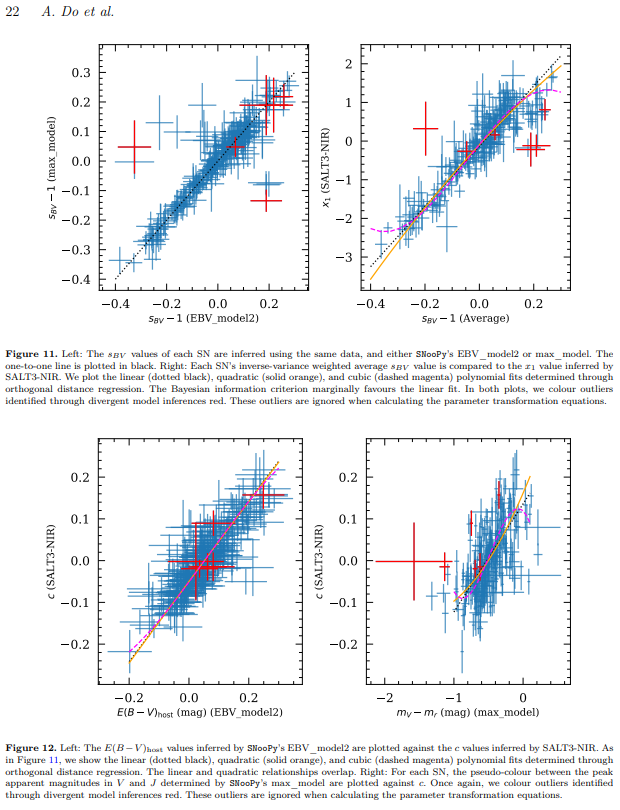
\includegraphics[width=1\textwidth]{images/snoopyvssalt.png}
    \centering
\end{frame}



\section{Time sensitive anomaly detection}

\begin{frame}{Time sensitive likelihood}
    \begin{itemize}
    \item Likelihood from before is extended into two dimensions, becoming
    \end{itemize}
    \begin{multline}\label{eq:time_sep_flagged}
    \log \mathcal{L} \left(\theta\right) = \sum_{ij} \left[\log \mathcal{L}_{ij} \left(\theta\right) + \log\left(1-p_{ij}\right)\right]\epsilon_{ij} +
    \\
    \left[ \log p_{ij} - \log \Delta \right]\left(1-\epsilon_{ij}\right)
    \end{multline}
  \end{frame}


  \begin{frame}{Time sensitive likelihood}
      \begin{itemize}
      \item Computation time of the likelihood grows linearly with the number of time bins used in the data set.
      \end{itemize}
      \begin{multline}\label{eq:time_sep_flagged}
      \log \mathcal{L} \left(\theta\right) = \sum_{ij} \left[\log \mathcal{L}_{ij} \left(\theta\right) + \log\left(1-p_{ij}\right)\right]\epsilon_{ij} +
      \\
      \left[ \log p_{ij} - \log \Delta \right]\left(1-\epsilon_{ij}\right)
      \end{multline}
    \end{frame}

  \begin{frame}
  \frametitle{Speeding up}

  % Start of the two-column layout
  \begin{columns}[T]

      % Left column for bullet points
      \begin{column}{0.5\textwidth}
          \begin{itemize}
              \item Anstey proposes a solution to this problem in~\cite{anstey2023use}
              \item Common model per time bin is fit jointly.
              \item Speeds up fit but not sensitive to transients.
          \end{itemize}
      \end{column}

      % Right column for screenshots
      \begin{column}{0.5\textwidth}
          \begin{figure}
              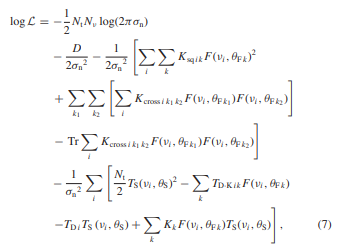
\includegraphics[width=\textwidth]{images/dom_timedep_math.png}
            \end{figure}
      \end{column}

    \end{columns}
      \begin{tikzpicture}[remember picture, overlay]
      \node [anchor=north east, inner sep=0pt] at ([xshift=-2.5cm, yshift=-1.1cm]current page.north east) {
          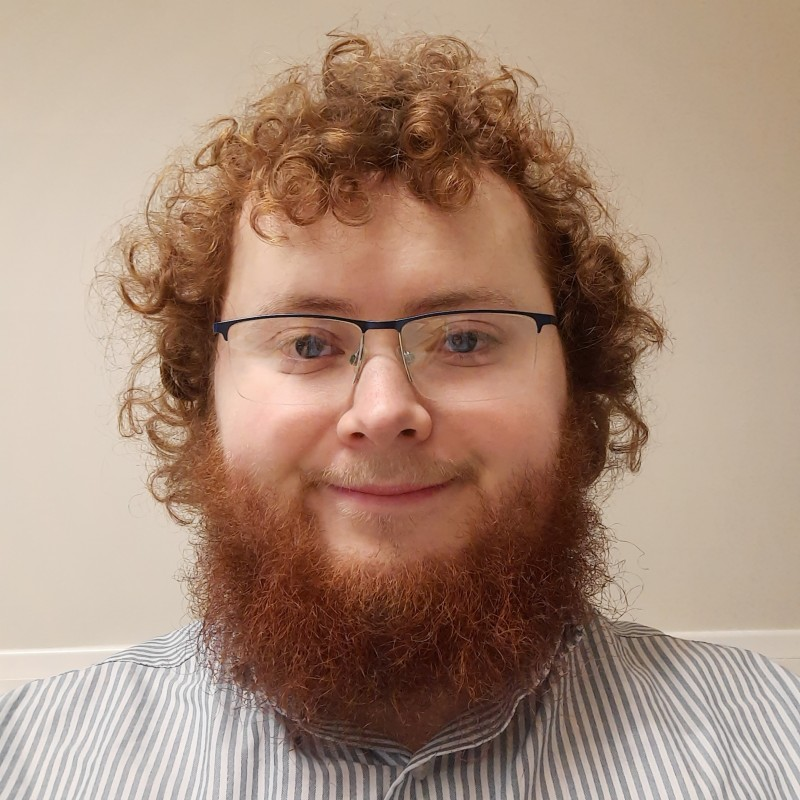
\includegraphics[width=1.7cm]{images/dom_pic.jpeg} % Adjust the size as needed
      };
      \end{tikzpicture}

    \end{frame}


    \begin{frame}
        \frametitle{Likelihood reweighting}

        \begin{columns}
            \begin{column}{0.5\textwidth}
                \begin{itemize}
                    \item Introduced in context of gravitational waves by \cite{payne2019higher} and \cite{romero2019searching}
                    \item Bayesian sampling techniques spend lots of time at tails of distribution.
                    \item Reweighting is essentially a coarse then fine search, using a simple (fast) then complex (slow) likelihood.
                \end{itemize}
            \end{column}
            \begin{column}{0.5\textwidth}
                \footnotesize
                \begin{align}
                    p(\theta|d) &= \frac{L(d|\theta)\pi(\theta)}{Z} = w(d|\theta) \frac{L_0(d|\theta)\pi(\theta)}{Z_0} \\
                    w(d|\theta) &\equiv \frac{L(d|\theta)}{L_0(d|\theta)} \\
                    Z &= Z_0 \int d\theta \, p_0(\theta|d) \left[ \frac{L(d|\theta)}{L_0(d|\theta)} \right] \\
                      &= Z_0 \sum_{k=1}^{n} w(d|\theta_k)
                \end{align}
                Carrying out Bayesian inference with the proposal likelihood, we obtain "proposal posterior samples" for the distribution
                \[
                    p_0(\theta|d) = \frac{L_0(d|\theta)\pi(\theta)}{Z_0}
                \]
            \end{column}
        \end{columns}
    \end{frame}

    \begin{frame}
      \frametitle{How does this help us?}
      \begin{columns}
      \begin{column}{0.5\textwidth}
        \begin{itemize}
          \item We can use the fast method for a coarse scan.
          \item Then the slower method for refined scan.
          \item Increases speed massively for larger problems.
      \end{itemize}
    \end{column}
    \begin{column}{0.5\textwidth}
      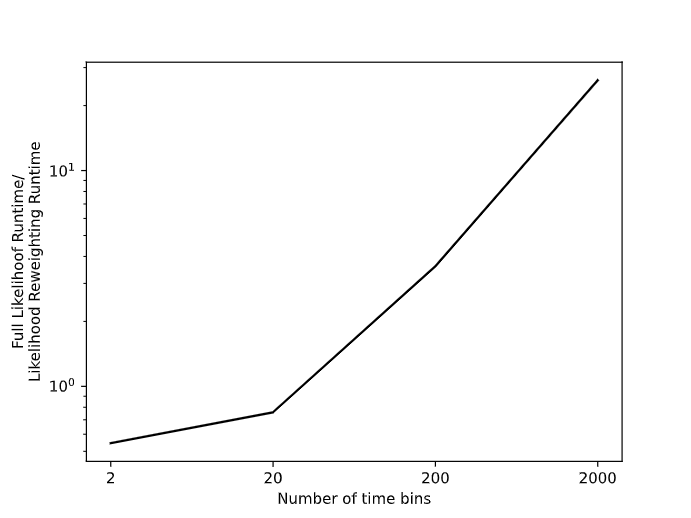
\includegraphics[width=1\textwidth]{images/lrw_runtime.png}
    \end{column}
  \end{columns}
  \end{frame}

    \begin{frame}
      \frametitle{Read the paper!}
      \begin{figure}
      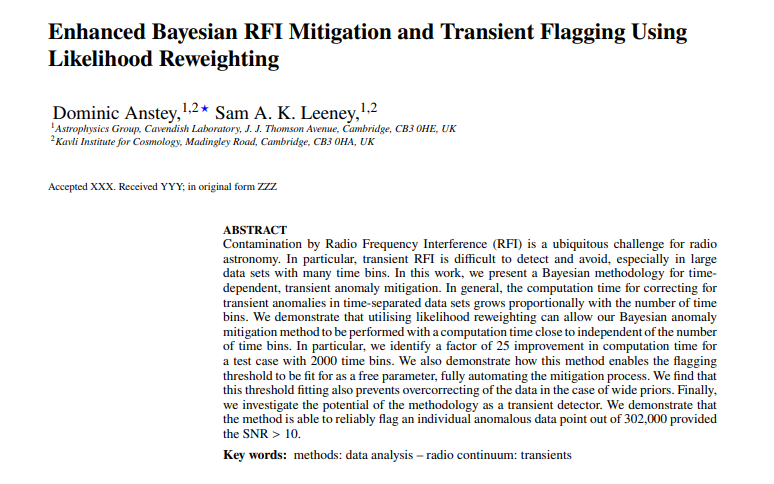
\includegraphics[width=0.7\textwidth]{images/da_sl_paper.png}
    \end{figure}
    \href{https://arxiv.org/abs/2310.02146}{arxiv: 2310.02146}

    \end{frame}

    \begin{frame}
      \frametitle{Conclusions}
      \begin{columns}
      \begin{column}{0.5\textwidth}
        \begin{itemize}
          \item Anomaly detection in the likelihood domain
          \item Simultaneous anomaly detection and mitigation
          \item Implement with 2 lines of code!
        \end{itemize}
    \end{column}
  \end{columns}
\end{frame}

  \begin{frame}[allowframebreaks]{References}
    \bibliography{ref}
  \end{frame}

\end{document}
